\documentclass[12pt]{article}
\usepackage[a4paper,bindingoffset=0.2in,%
            left=1in,right=1in,top=1in,bottom=1in,%
            footskip=.25in]{geometry}
\title{User Guide}
\author{Group 15}
\usepackage{listings}
\usepackage{color}
\usepackage{graphicx}


\definecolor{dkgreen}{rgb}{0,0.6,0}
\definecolor{gray}{rgb}{0.5,0.5,0.5}
\definecolor{mauve}{rgb}{0.58,0,0.82}

\lstset{frame=tb,
  language=Java,
  aboveskip=3mm,
  belowskip=3mm,
  showstringspaces=false,
  columns=flexible,
  basicstyle={\small\ttfamily},
  numbers=none,
  numberstyle=\tiny\color{gray},
  keywordstyle=\color{blue},
  commentstyle=\color{dkgreen},
  stringstyle=\color{mauve},
  breaklines=true,
  breakatwhitespace=true,
  tabsize=3
}
\begin{document}
\graphicspath{ {images/} }
	\maketitle
	\setlength{\parindent}{0pt}
\pagenumbering{gobble} 

 \section{Installation} 
  \bigskip
 

 \subsection{How to install from Github and set up} 
 
 \begin{lstlisting}
	$ git clone https://github.com/julijonas/venus.git
\end{lstlisting}
	Python part:
	\begin{lstlisting}
	$ cd sdp
	$ virtualenv env
	$ source env/bin/activate
	$ pip install -r requirements.txt
	
	\end{lstlisting}

	Arduino part:
	\begin{lstlisting}
	$ arduino
	\end{lstlisting}
	You'll need to add three libraries (can be found under arduino/ in the project directory): ArduinoSerialCommand, SDPArduino, SimpleTimer
	\bigskip

	In order to add a library go to: 
	\begin{lstlisting}
	Sketch -> Import Library... -> Add Library... and choose the library folder you want to import.
	\end{lstlisting}

\section{Overview of the robot}
        At the current stage, our robot - Venus - can move and kick. It moves because it has wheels connected to NXT motors, and we can send commands that power the certain motors on and off (depending which action we want the robot to make). The kicker is also connected to the NXT motor, which allows us to control the power of the kick. 
      
	\subsection{Use}
	In order to turn the robot on, connect the battery pack to the board. 
        In order to swap batteries, take them out, put them charging and put new batteries into the battery pack. Easy!

\section{Running Instructions} 
   (To be changed after the first milestone)
   \bigskip 
   
   Run the command in the terminal from the project root directory: 
			\begin{lstlisting}
			source env/bin/activate
			\end{lstlisting}
   Then in order to send the commands the robot: 
			\begin{lstlisting}
			python control/control.py
			\end{lstlisting}
   After that you should be able to send commands to the robot (make sure the usb stick is plugged in).
   \bigskip
   
   \textbf{NB} In case you make changes to Arduino code, you should upload the changes to the board!
   \bigskip
   
   The list of possible commands is below:
	\bigskip
	\begin{itemize}
  \item For moving to the target in the milestone 1, there is a command 'move'.
  \bigskip
  
	At the begging the robot turns 90 degrees to the right (if "distance1" parameter is positive the robot will move to the forwards, if negative backwards). After covering the first distance it turns 90 degrees so that it faces the same way as at the start. The "degrees" parameter is amount of degrees the robot turns (positive - clockwise, negative - anticlockwise)
	\bigskip
	
		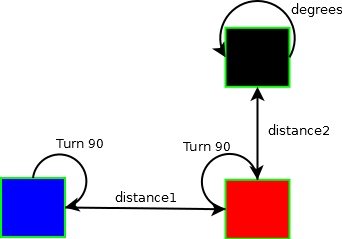
\includegraphics{Diagram1}
		
		\begin{lstlisting}
		 move <distance1> <distance2> <degrees>
		\end{lstlisting}
\newpage

 	  \item For kicking:
		\begin{lstlisting}
	    kick [50|100|150]
		\end{lstlisting}
	\item For moving forward and turning:
		\begin{lstlisting}
	    f <distance>
		 c <degrees>
		\end{lstlisting}
\end{itemize}
		
\section{Troubleshooting guide}
	\textbf{Problem 1} When trying to upload the code to the Arduino board, you get the error message below.
	\begin{lstlisting}
	processing.app.SerialNotFoundException: Serial port '<port>' not found. Did you select the right one from the Tools > Serial Port menu?
	\end{lstlisting}
	
	\bigskip
	
	\textbf{Solution}  It can't detect the Arduino board. Make sure it's connected to the computer through the USB stick or the cable. If it is, disconnect and connect again, or power the board off and on again. Make sure you are not running 'python control/control.py' when you're uploading the changes.
	\bigskip

	\textbf{Problem 2} When sending commands the robot doesn't do anything and you're sure it should move.
	\bigskip
	
	\textbf{Solution} Power the Arduino board off and on again.

 
\end{document}